% BOF Preamble
\documentclass[cmpstyle]{ueacmpstyle}
% imports
\usepackage{fancyhdr}
\usepackage{csquotes}
\usepackage{wrapfig}
\pagestyle{fancy}
\fancyhead{}
\fancyfoot{}
\lfoot{100036248}
\rfoot{Page \thepage}
\renewcommand{\footrulewidth}{0.4pt}
% macros
% EOF Preamble

% BOF Document
\begin{document}
	\title{Much ado about Everything: \\ The Configuration Management Story}
	\author{Christopher A. Irvine}
	\date{\today}
	\maketitle
	
	\begin{abstract}
		200 words of text here about how awesome this is
	\end{abstract}

	\section{Introduction} \label{sec:intro}
	Configuration Management (CM) has helped many organisations across the globe manage the development and maintenance of complicated systems. However, the influence of CM does not stop in the office. The techniques used to incorporate the CM functions into a project have seeped out into every day life. In a similar manner, CM has taken many every day organisational techniques to heart. 
	
	In this paper we will look at where CM originated from and how it has evolved to be relevant in the industries of today (see Section \ref{sec:history}). Then we will look how the functions of CM (see Section \ref{sec:principles}) are used both in the office and at the home (see Section \ref{sec:using}). Before performing a critical analysis on the benefits gained from incorporating CM into a project or personal life, to try to justify the costs associated with that incorporation (see Section \ref{sec:embracing}). 
	
		\subsection{Defining Configuration Management (CM)} \label{sec:definition}
		Before we continue to answer the questions outlined in Section \ref{sec:intro}, we should have an understanding of what the modern definition of CM is. 
		
		According to the \emph{Association of Project Management (APM)}: 
		
		\begin{quote}
		``Configuration Management encompasses the administrative activities concerned with the creation, maintenance, controlled change and quality control of the scope of work." (\cite{apmDef})
		\end{quote}
		
		Expanding upon this definition; CM is a collection of principles, techniques and characteristics that aim to control the execution of a project. This allows for the Project Manager to ensure that all work regarding the project is of a high quality by deploying CM techniques, ensuring that short-term targets and long-term goals are achieved.
	
	\section{History of CM} \label{sec:history}
	In this section we will take a brief look at where CM came from and why it was created (see Section \ref{sec:origin}), and how CM spread across the globe (see Section \ref{sec:adoption}). Finally we will learn how the CM has evolved to remain relevant in the IT industry, and what standards have emerged as a result.
	
		\subsection{Origins} \label{sec:origin}
		The origins of CM can be traced back to the U.S. Department of Defence (DoD), where the need for universal hardware standards was required in order to make maintenance of the equipment manageable. This was driven due to the mass of weapons and vehicles built during the second world war that were each unique and had its own set of issues. No two guns or tanks were the same. This meant the DoD was spending an excessive amount of money on training mechanics to maintain the equipment. The standards was created to save money and increase efficiency.
		
		\begin{wrapfigure}{l}{5cm}
			\centering
			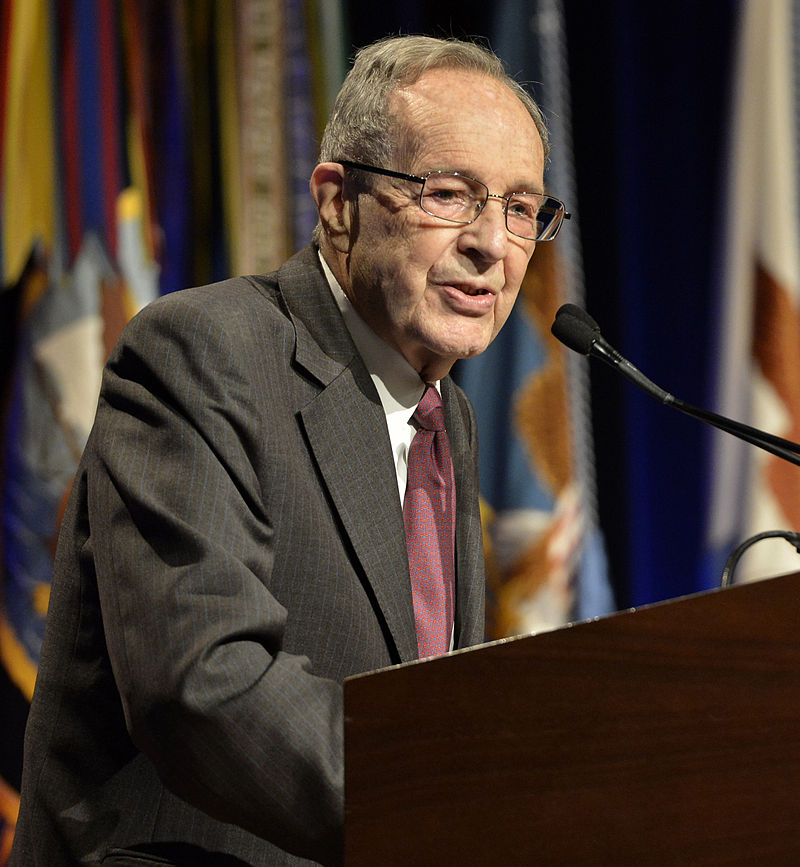
\includegraphics[height=4cm]{images/william-perry.jpg}
			\caption{William J. Perry, 19th Secretary of Defence for the United States under President Bill Clinton. Perry was instrumental in streamlining the US military infrastructure. Which formalised the discipline known as Configuration Management in private sector industries.}
		\end{wrapfigure}
	
		It was not until the 1960s that CM became a technical discipline of its own, when the DoD released a series of military standards known as the \emph{``480 series"}. These standards were regularly updated and eventually consolidated into MIL-HDBK-61 in 1991, which contained a series of technical standards supported by standards developing organisations (SDO)(personal communication, \cite{dod-history}) \footnote{A Standards Developing Organisation (SDO) is a body whose primary activities revolve around the improvement and development of technical standards within a given field (\cite{history-standards}).}.
		
		\subsection{Adoption into Industry} \label{sec:adoption}
		SDOs regulated their own industries through a collection of standards publications starting in the late 80s and early 90s. These various issues have evolved into a widely distributed an accepted standard on CM known as \emph{ANSI-EIA-649-1998 (EIA-649)}, a venture helmed by the Electronic Industries Alliance (EIA). EIA-649 has provided the base for many specialised CM techniques since the 90s, but this document describes the five primary functions of CM (\cite{EIA-649}). 
		
		\subsection{Software Configuration Management (SCM)} \label{sec:scm}
		Software Configuration Management evolved from the practices of the late 60s when Professor Leon Pressor wrote a thesis on change and configuration control, whilst working with the DoD. He took the some of the basic concepts of CM, which are discussed in Section \ref{sec:principles}, and revised others into tools and techniques that solve the issues that were occurring during software projects. This created a set of distinct emphases that were separate from the emphases in traditional CM.
		
	\section{The 5 Functions of CM/SCM} \label{sec:principles}
	EIA-649 (see Section \ref{sec:adoption}) outlines 5 functions (sometimes known as disciplines) that should be enforced in both hardware and software projects. Together they establish a standard for managing the development of a project (\cite{mil-hdbk}). 
	
	This section will take a brief look at the 5 traditional functions of CM before looking how they differ in SCM, as detailed by the latest version of EIA-649.
	
		\subsection{CM Planning and Management} \label{sec:planning}
		Each project should have a formal document that outlines, in detail, all process that are required for the project. This should be used as a reference for everyone involved. Such a document will include procedures for:
		\begin{itemize}
			\item personnel
			\item responsibilities and resources
			\item training
			\item administrative meeting guidelines
			\item base lining resources (see Section \ref{sec:identify})
			\item configuration control and configuration status accounting (see Sections \ref{sec:control} and \ref{sec:accounting})
			\item naming conventions
			\item audits and reviews (see Section \ref{sec:audit})
			\item subcontractor/vendor CM requirements
		\end{itemize}
		These processes will be created before development of the project has begun. Any changes to this document during the life-cycle of the project should be avoided, to prevent confusion. But if changes are needed, then a Document Change Notice (DCN) should be issued to all personnel. The details of a DCN can be found within a CM document.
		
		\subsection{Configuration Identification (CI)} \label{sec:identify}
		CI involves defining the system and subsystem architectures through the use of baselines. The procedures for changing any part of the system - how the change is identified, documented and tracked through design, development, testing and delivery - is created during this function. 
		
		\subsection{Configuration Control} \label{sec:control}
		Configuration Control is the evaluation of all change-requests and change-proposals to the project and its documentation; including the process for approving or rejecting the changes.
		
		\subsection{Configuration Status Accounting} \label{sec:accounting}
		Configuration Status Accounting dictate the process for recording and reporting configuration item descriptions and all changes from the original designed baseline.
		
		\subsection{Configuration Verification and Audit} \label{sec:audit}
		The final function of CM is the independent review of hardware and software to ensure that the product meets the established performance requirements outlined at the start of the project.
		
		\subsection{Alterations for SCM} \label{sec:scm-alterations}
		SCM was created to better suit the challenges posed by Software Projects, as stated in Section \ref{sec:scm}. SCM places a greater emphasis on the need to trace changes in the system with the ability to verify that the delivered software does not exceed the original intent for the program. As a result the four functions for SCM are:
		
		\begin{enumerate}
			\item Configuration Identification (CI)
			\item Configuration Change Control
			\item Configuration Status Accounting
			\item Configuration Audits
		\end{enumerate}
	
		The first three functions of SCM are closely linked to their traditional counterparts, see Sections \ref{sec:identify}, \ref{sec:control} and \ref{sec:accounting} for details about SCM 1, 2 and 3. 
		
		Configuration Audits for SCM are separated into two halves, functional and physical, both of which can occur at either delivery or when a change is implemented. Functional audits look at a configuration item to ensure that it meets both the functional and performance requirements. A physical audit ensures that a configuration item is installed within the wider system in accordance with the system design documentation .
		
		Notice that the CM Planning and Management function of traditional CM has been entirely removed from SCM. That is because Design Document, a Software Engineering practice, covers the majority of the same topics \footnote{A Design Document is a technical guide for Developers to use before, during and after Developing a piece of Software.}(\cite{DesignDocExample}).
		
	\section{Using CM} \label{sec:using}
	
		\subsection{In the Office} \label{sec:office}
		
		\subsection{At Home} \label{sec:home}
		
	\section{Embracing CM} \label{sec:embracing}
	
		\subsection{Benefits of CM} \label{sec:benefits}
		
		\subsection{Costs} \label{sec:costs}
		
	\section{Conclusion} \label{sec:conc}
	
	\bibliographystyle{apalike}
	\bibliography{report}
\end{document}

% EOF Document